\documentclass[laurea,oneside,11pt]{report}
\usepackage{graphicx}
\usepackage{subfigure}
% \usepackage[latin1]{inputenc}
\usepackage[italian]{babel}
\usepackage[utf8]{inputenc}
\usepackage{amsfonts}
\usepackage{amsmath} % assumes amsmath package installed
\usepackage{amssymb}  % assumes amsmath package installed
\usepackage[pagestyles]{titlesec}
\usepackage{algorithm,algpseudocode}
% \usepackage{hyperref}
\usepackage{float}
\usepackage{rotating}
\usepackage{url}
% \usepackage{cite}
\usepackage{color}
\usepackage{epstopdf}
\usepackage{listings}
\usepackage{xcolor}
\usepackage{latexsym}
\usepackage{psfrag}
\usepackage{fancyhdr}

\usepackage[nokeyprefix]{refstyle}
\usepackage{varioref}
\usepackage{xr-hyper}
\usepackage[hidelinks]{hyperref}

\usepackage{textcomp}
\usepackage{multirow}
\usepackage{booktabs}






\setcounter{secnumdepth}{5}
\setcounter{tocdepth}{5} 
\DeclareMathOperator*{\argminB}{argmin}

\usepackage[margin=4cm]{geometry}
\newcommand{\HRule}{\rule{\linewidth}{0.5mm}} % Defines a new command for the horizontal lines, change thickness here

\begin{document}

\begin{titlepage}


%----------------------------------------------------------------------------------------
%	LOGO SECTION
%----------------------------------------------------------------------------------------
\center % Center everything on the page
 \includegraphics*[width=0.5\columnwidth]{Logo}~\\[.5cm]
%----------------------------------------------------------------------------------------
%	HEADING SECTIONS
%----------------------------------------------------------------------------------------

\textsc{\LARGE Universita' di Pisa}\\[1.0cm] % Name of your university/college
\textsc{\Large Ingegneria Robotica}\\[0.5cm] % Major heading such as course name
\textsc{\large Sistemi di guida e navigazione}\\[0.5cm] % Minor heading such as course title

%----------------------------------------------------------------------------------------
%	TITLE SECTION
%----------------------------------------------------------------------------------------

\HRule \\[0.3cm]
{ \huge \bfseries Algoritmo di tracking per la stima della posa di una camera monoculare}\\[0.4cm] % Title of your document
\HRule \\[1.cm]
 
%----------------------------------------------------------------------------------------
%	AUTHOR SECTION
%----------------------------------------------------------------------------------------

\begin{minipage}{0.4\textwidth}
\begin{flushleft} \large
\emph{Studente:}\\
Daniela \textsc{Resasco} % Your name
\end{flushleft}
\end{minipage}
~
\begin{minipage}{0.4\textwidth}
\begin{flushright} \large
\emph{Professore:} \\
Lorenzo \textsc{Pollini}  % Supervisor's Name
\end{flushright}
\end{minipage}\\[4cm]

%----------------------------------------------------------------------------------------
%	DATE SECTION
%----------------------------------------------------------------------------------------
{\large \today}\\[3cm] % Date, change the \today to a set date if you want to be precise

 
%----------------------------------------------------------------------------------------

\vfill % Fill the rest of the page with whitespace
\end{titlepage}
% \begin{flushleft}



\pagenumbering{roman}
\newpage 
\section*{Abstrac} % (fold)
\label{sec:abstract}
In questo report verrà presentato l'algoritmo di visione implementato per la stima della posa di una camera monoculare. Queste informazioni verranno utilizzate in seguito per il controllo di un braccio robotico posto su di una carozzina al fine di premere un pulsante scelto dall'utente. 
Il pulsante viene premuto dall'utente tramite interfaccia tablet. Una volta identificato il pulsante premuto, la camera fornisce al robot le informazioni di posizione ad orientazione dello stesso, in modo da posizionarsi sul percorso corretto. La camera utilizzata è monoculare pertanto non si hanno informazioni sulla distanza. Per ovviare a questa mancanza si è deciso di utilizzare un algoritmo esterno capace di utilizzare le informazioni delle features trovate per stimare la posizione relativa. Questo algoritmo è affetto da un errore di scala e per ridurne gli effetti, si utilizza un criterio di convergenza della stima del fattore di scala utilizzando il metodo della massima verosimiglianza.  

\newpage 
% % % % % Indice % % % % %
% \frontmatter
% \pagenumbering{roman}
\tableofcontents
\newpage 
\listoffigures
% \newpage

% \newpage 
% \section*{Abstrac} % (fold)
% \label{sec:abstract}
% In questo report verrà presentato l'algoritmo di visione per la stima della posa di una camera monoculare. Queste informazioni verranno utilizzate in seguito per il controllo di un braccio robotico posto su di una carozzina al fine di premere un pulsante scelto dall'utente. 
% Il pulsante viene premuto dall'utente tramite interfaccia tablet. Una volta identificato il pulsante premuto, la camera fornisce al robot le informazioni di posizione ad orientazione dello stesso, in modo da posizionarsi sul percorso corretto. La camera utilizzata è monoculare pertanto non si hanno informazioni sulla distanza. Per ovviare a questa mancanza si è deciso di utilizzare un algoritmo esterno capace di utilizzare le informazioni delle features trovate per stimare la posizione relativa. Questo algoritmo è affetto da un errore di scala e per ridurne gli effetti, si utilizza un criterio di convergenza della stima del fattore di scala utilizzando il metodo della massima verosimiglianza.  



\newpage 
\clearpage
\pagenumbering{arabic}
% \mainmatter
%!TEX root = pag0.tex

\chapter{Introduzione}
\label{chapter1}
%In questo report verrà presentato il progetto del corso di Guida e Navigazione. 
Nella vita quotidiana ci troviamo spesso a dover premere dei pulsanti, i.e quelli del citofono, i pulsanti dell'ascensore etc. Le pulsantiere, si pensi a quelle degli ascensori, sono poste in modo da essere premute senza dover alzare il braccio più in alto della linea degli occhi. Se pensiamo ai bambini, per premere un pulsante si mettono sulle punte dei piedi. Cosa succede se una persona con una carrozzina non arriva a premere un pulsante?. Questo progetto si occupa di aiutare i diversamenti abili ad essere più indipendenti. Lo scopo del progetto è l'identificazione della posizione del pulsante desiderato e l'invio di tali informazioni al controllore del braccio robotico. L'utente con il supporto di un tablet, preme su di esso il bottone desiderato. Una volta identificato il pulsante premuto, la camera fornisce al robot le informazioni di posizione ad orientazione in modo da posizionarsi sul percorso corretto. La camera utilizzata è monoculare pertanto non si hanno informazioni sulla distanza. Per ovviare a questa mancanza si è deciso di utilizzare un algoritmo esterno chiamato \emph{PTAM} ~\cite{PTAM} capace di utilizzare le informazioni delle features trovate per stimare una posizione relativa.
Il codice si divide in tre fasi:
\begin{itemize}
\item Fase di plan
\item Fase di tracking
\item Interfacciamento con l'algoritmo esterno
\item Fase di triangolazione e scalatura
\end{itemize}
Nella prima fase si utilizzano algoritmi di elaborazione dell’immagine, in modo da ottenere la posizione
dell’oggetto in coordinate camera. Nella seconda fase si ricercano nella seconda immagine le features di interesse e si stima la posizione del bottone tramite algoritmi di matching. Nella terza fase si elaborano i dati ricevuti dall'algoritmo esterno, Ptam. Nella quarta e ultima fase i dati elaborati vengono triangolati e, opportunamente scalati per trovare la posa relativa.

I sistemi di acquisizione maggiormente impiegati possono essere suddivisi in due categorie. Una prima categoria fa riferimento al modo in cui viene usato il sistema di visione. Se la telecamera inquadra direttamente l’oggetto dal punto di vista del manipolatore, si parla di sistemi \lq \lq eye-in-hand \lq \lq. In questo caso la posizione
e l’orientamento della telecamera sono solidali con l’end-effector del manipolatore.
Un’altro tipo di configurazione consente di avere la telecamera che mantiene una posizione fissa nell’ambiente e al più con orientamento variabile, ed inquadra sia il manipolatore che l’oggetto target. Quest’ultima modalità
viene denominata \lq \lq eye-to-hand \lq \lq.. È possible notare le differenze nelle capacità visive del manipolatore in questa due modalità di configurazione dalla figura ~\ref{fig:eye_in_hand}
\begin{figure}[H]
   \centering
   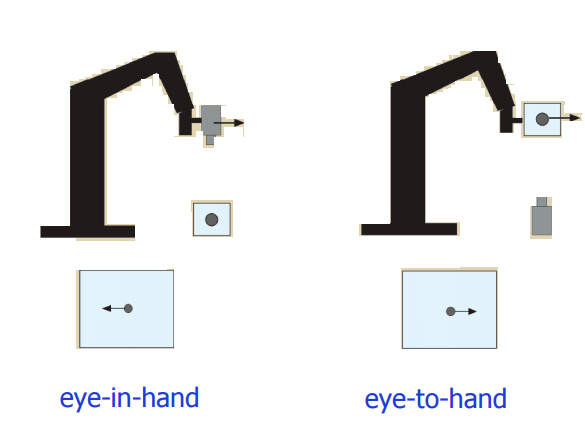
\includegraphics[width=.7\columnwidth]{eyetoinhand.png}
   \caption{Differenza tra le due categorie di posizionamento della camera}
   \label{fig:eye_in_hand} 
\end{figure}
Nelle tecniche tradizionali di asservimento visivo viene invece spesso effettuata la misura diretta della posizione del manipolatore fornita dalla telecamera, per migliorare l’accuratezza del posizionamento del end-effector. I dati forniti dalla telecamera, in questo caso, incrementano la precisione delle informazioni fornite dall’apparato meccanico del robot, in quanto non risultano affetti dai tipici errori dovuti ad un’imprecisa conoscenza dei parametri fisici del manipolatore, che risultano particolarmente evidenti nel caso in cui si debba considerare anche la flessibilità della struttura.
L’ambiente, in cui si muove il robot, possiede alcune caratteristiche che inevitabilmente influenzano il processo di comprensione della scena. Nei sistemi robotici dotati di sensori di visione vengono spesso applicate le seguenti ipotesi:
\begin{itemize}
\item il robot deve essere un agente autonomo, per cui non è possibile alcun intervento esterno per controllarlo;
\item gli oggetti da riconoscere presenti nell’immagine devono essere fortemente caratterizzati;
\item le condizioni di illuminazione della scena sono in genere fortemente variabili, questo influisce molto sul riconoscimento degli oggetti;
\item le occlusioni, rendono impossibile il riconoscimento degli oggetti basandosi sull’analisi della loro forma
\end{itemize}
In questo progetto è stato impiegato una configurazione del primo tipo. 





% \newpage 



\subsection{Organizzazione del report}
Nel capitolo ~\ref{chapter2} si spiega il modello della camera utilizzata e le sue caratteristiche.  Nel capitolo ~\ref{chapter3} verrà spiegato il meccanismo di tracking e del matching mentre nel capitolo ~\ref{chapter4} viene introdotto l'algoritmo sviluppato. Nel capitolo ~\ref{chapter5} vengono esposti gli esperimenti e nel ~\ref{chapter6} le conclusioni. In appendice A vi è una panoramica del codice sviluppato. 
% Include the first content chapter
%!TEX root = pag0.tex

\chapter{Modello della camera}
\label{chapter2}


La camera utilizzata è una camera monoculare posta sul end-effector del braccio robotico. Questo tipo di telecamera ha un ingombro minimo, ma si perde la percenzione della distanza. Per ricostruire queste informazioni occorre utilizzare la \emph{stereo visione}\footnote{Stima della profondità tramite l'utilizzo di due immagini della stessa scena prese da angolazioni differenti} utilizzando la \emph{geometria epipolare} \footnote{Essa descrive le relazioni e i vincoli geometrici che legano due immagini 2D della stessa scena 3D catturata da due fotocamere con posizione e orientamento distinto}. 
La camera utilizzata nel progetto è la camera monoculare della Playstation 3 mostrata in Fig ~\ref{fig:camera} di produzione della Sony con una risoluzione di 640X480 pixel. 
\begin{figure}[H]
   \centering
   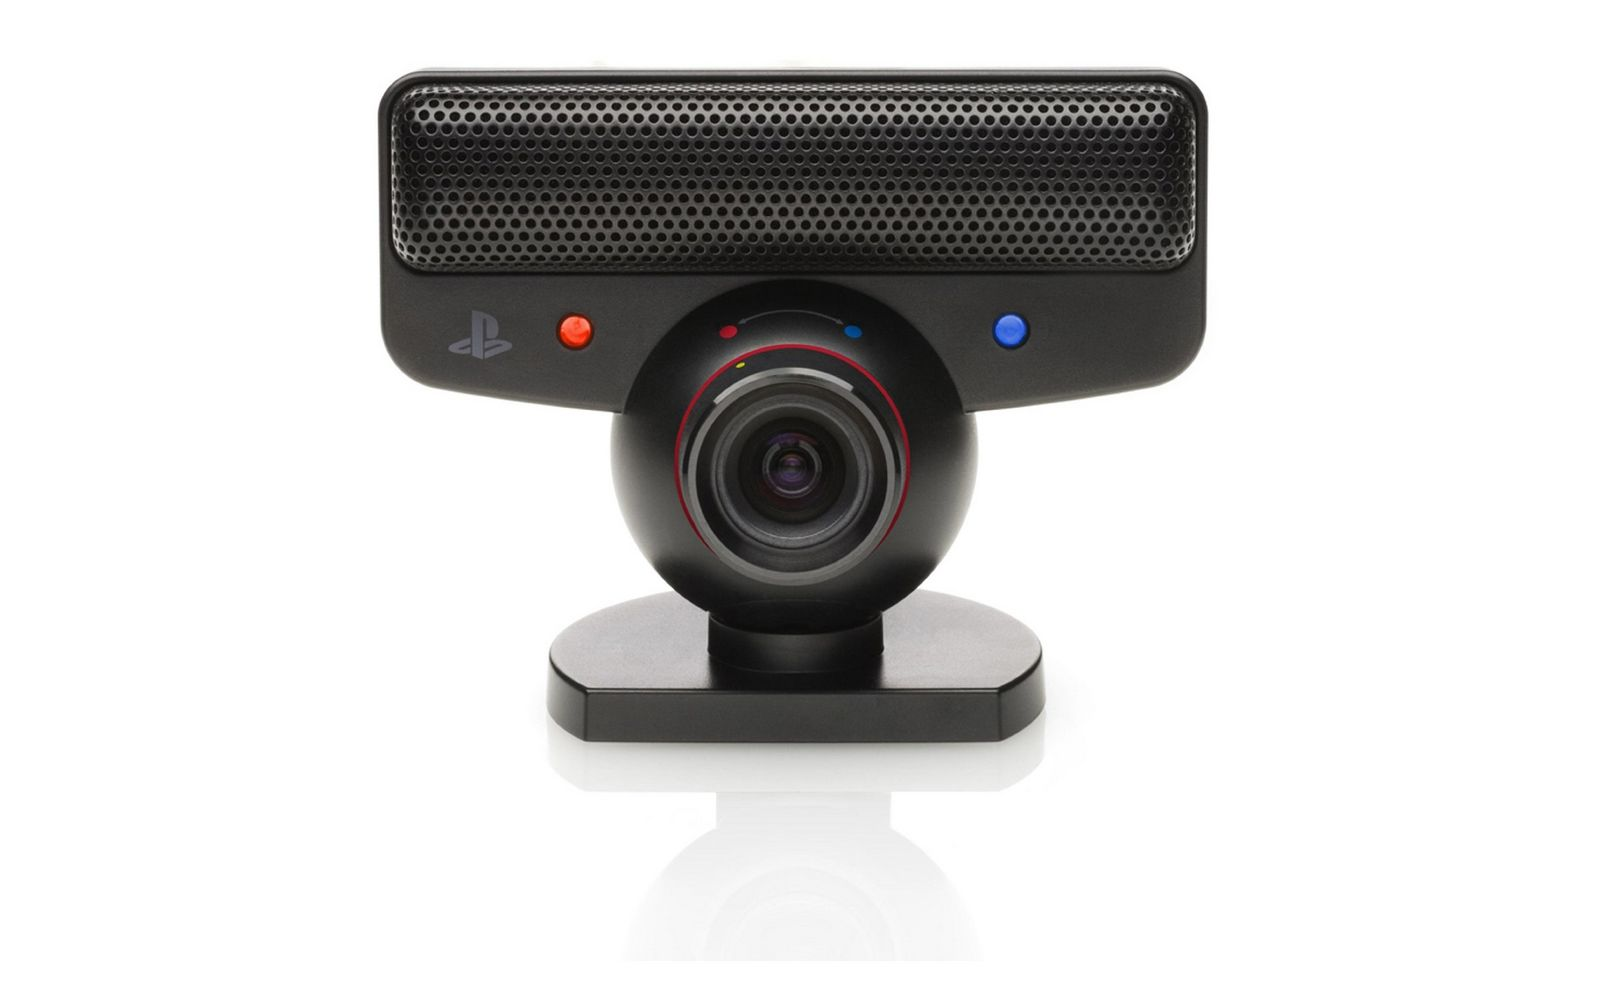
\includegraphics[width=.7\columnwidth]{camera.jpg}
   \caption{Camera utilizzata nel progetto}
   \label{fig:camera} 
\end{figure}


\newpage 
\subsection{Modello pinhole}
La geometria di tale modello prevede che i raggi luminosi provenienti dal mondo che passano attraverso un foro di dimensione infinitesima, vadano a formare l'immagine su un piano disposto dietro il foro, chiamato \emph{piano immagine}. In termini matematici consideriamo un punto nel mondo con cordinate $X_c = [X_c, Y_c, Z_c]^T $ il cui sistema di riferimento $O$ è centrato nel foro. Questo sistema di riferimento prende il nome di \emph{centro ottico}. L'asse $z$ è l'asse ottico, ed è la retta perpendicolare al piano dell'immagine passante per il centro ottico. Il raggio luminoso che segue l'asse ottico è chiamato \emph{raggio principale}. La distanza fra il piano immagine e il centro ottico è la \emph{lunghezza focale} $f$. La figura ~\ref{fig:pinhole} mostra lo schema di queste definizioni.
\begin{figure}[H]
   \centering
   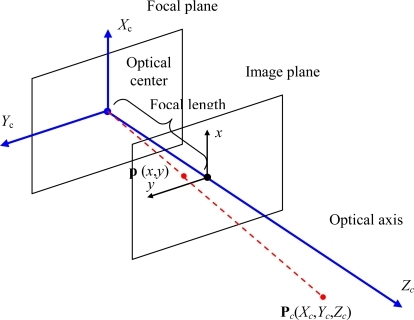
\includegraphics[width=.7\columnwidth]{pinhole.png}
   \caption{Modello schematico del modello pinhole}
   \label{fig:pinhole} 
\end{figure}
Con queste definizioni possiamo chiamare \emph{parametri instrinseci} tutti quei parametri necessari a collegare le coordinate di un pixel dell'immagine con le coordinate corrispondenti nel sistema di riferimento della camera. In altre parole sono i parametri necessari a specificare le caratteristiche ottiche, geometriche e digitali della camera. Tali parametri sono:
\begin{itemize}
\item la lunghezza focale
\item le coordinate in pixel del centro dell'immagine
\item la distorsione geometrica 
\item la dimensione dei pixel
\end{itemize}
I \emph{parametri estrinseci} sono tutti quei parametri che definiscono la posizione ed orientazione del sistema di riferimento della camera rispetto al riferimento mondo. Sono un insieme di parametri geometrici che identificano univocamente le trasformazioni tra il sistema di riferimento della camera e quello mondo, supposto noto. Tali parametri sono:
\begin{itemize}
\item vettore di traslazione
\item matrice di rotazione 3x3 ortogonale
\end{itemize}
Il punto sul piano immagine $x = [x_i,y_i]^T$ corrispondente a $X_c$ è definito come in figura ~\ref{fig:images_point} 
\begin{figure}[H]
   \centering
   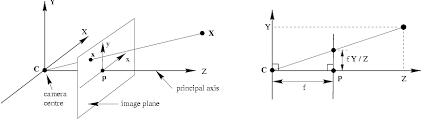
\includegraphics[width=1\columnwidth]{images_point.png} 
   \caption{Punti nel piano immagine}
   \label{fig:images_point} 
\end{figure}
\begin{equation}
\begin{cases}
x_i = f_x * \frac{X_c}{Z_c}	+ c_x\\	
y_i = f_y* \frac{Y_c}{Z_c} + c_y
 \end{cases}
\label{eq:punto_immagine}
\end{equation}
Utilizzando il modello pinhole, il punto $X_c$ proiettato nel piano immagine è esprimibile come:
\begin{equation}
 s* \begin{bmatrix}
    x  \\
    y \\
    1
  \end{bmatrix} = \begin{bmatrix}
    f_x & 0&c_x  \\
    0&f_y&c_y \\
    0&0&1
  \end{bmatrix} * \begin{bmatrix}
  r_{11} & r_{12} & r_{13} & t_1 \\
  r_{21} & r_{22} & r_{23} & t_2	\\
  r_{31} & r_{32} & r_{33} & t_{3}
  \end{bmatrix} *\begin{bmatrix}
    X_c  \\
    Y_c \\
    Z_c \\
  \end{bmatrix}
\label{eq:punto omogeneo}
\end{equation}
Dove $c_x$ e $c_y$ sono i centri ottici espressi in pixel e $A$ è la matrice dei parametri intrinseci, il fattore $s$ che moltiplica il vettore dei punti nel piano immagine è detto \emph{fattore di scala}. La matrice di roto-traslazione è chiamata matrice dei parametri estrinseci, ed è usata per descrivere il moto della camera attorno ad una scena statica. Nella figura ~\ref{fig:modello_pin} si può vedere uno schema del modello pinhole con la descrizione dei parametri intrinseci ed estrinseci.
\begin{figure}[H]
   \centering
   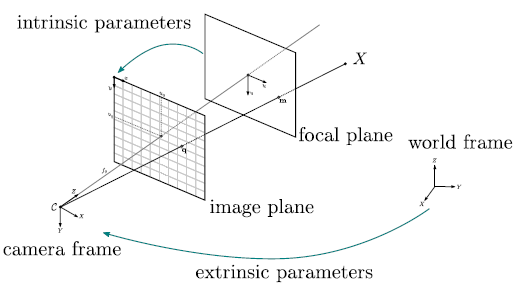
\includegraphics[width=0.7\columnwidth]{pinholeCamera.png} 
   \caption{Schema del modello pinhole con parametri estrinseci ed intrinseci}
   \label{fig:modello_pin} 
\end{figure}



 % Include the second content chapter
%!TEX root = pag0.tex
\chapter{Tracking and Matching tramite SIFT}
\label{chapter3}

Il tracking è l'operazione di seguire lo spostamento di un oggetto o di un insieme di punti in frame consegutivi. I punti usati per questa operazioni vengono chiamati \emph{features}. La qualità del tracking influenza in maniera molto significativa gli algoritmi che lo utilizzano. Nel codice sviluppato, il tracking viene utilizzato per stimare la posizione delle features dato il loro moto. 
Per lo studio in esame si è deciso di usare il tracking con il \emph{SIFT} acronimo di Scale-Invariant Feature Transform. Gli operatori utilizzati tradizionalmente in fotogrammetria (Forstner e Gulch 1988 ~\cite{Forstner}; Harris e Stephens 1988 ~\cite{Harry}) ricercano punti omologhi (point detector) su spigoli o discontinuità radiometriche; al contrario l’operatore SIFT ricerca i punti (keypoint) su regioni più ampie dell’immagine (region detector) superando i problemi di occlusione e deformazione prospettiche.
Questo metodo è stato sviluppato da D. G. Lowe ~\cite{Sift} e permette di rilevare i punti caratteristici di una immagine e di associargli dei descrittori basati sui gradienti delle aree dell'immagine nell'intorno delle features. Questi descrittori sono utilizzati per ricercare il punto nelle immagini successive.
I passi principali dell’algoritmo SIFT sono i seguenti:
\begin{itemize}
  \item Individuazione degli estremi locali nello scale-space: si cercano punti interessanti su tutte le scale e posizioni dell’immagine utilizzando una funzione DoG -Difference of Gaussian-. L’approccio utilizzato è quello del filtraggio in cascata (cascade filtering approach), che consente di determinare le posizioni e la scala delle features candidate ad essere punti chiave e che, in un secondo momento, vengono caratterizzate con maggior dettaglio.
  \item Localizzazione dei keypoint: per ciascun punto candidato viene costruito un modello dettagliato per determinarne posizione e scala. I punti vengono inoltre selezionati secondo misure di stabilità.
  \item Generazione delle orientazioni: per ottenere l’invarianza rotazionale, ad ogni punto chiave (keypoint) vengono associate una o più orientazioni calcolate in base ai gradienti locali dell’immagine.
  \item Generazione del descrittore: a partire dai gradienti locali dell’immagine, alla scala selezionata e nell’intorno del punto chiave, viene costruito il descrittore.
\end{itemize}
Lo scale-space è una funzione che permette di calcolare punti dell’immagine che sono invarianti a cambiamenti di scala definito come una funzione $L(x,y,\sigma)$ data dalla convoluzione in $x$ e $y$ di una funzione Gaussiana, variabile in scala, $G(x,y,\sigma)$ con l’immagine $I(x,y)$:
\begin{equation}
L(x,y,\sigma) =  G(x,y,\sigma) \otimes I(x,y)
\label{eq:surface_modeling}
\end{equation}
Ogni immagine è filtrata mediante convoluzioni di gaussiane, formando uno spazio delle \lq \lq scale \lq \lq. Per ogni scala sono quindi calcolate le differenze fra gaussiane adiacenti DoG, i cui massimi sono memorizzati come punti di interesse \emph{keypoints} ~\ref{fig:scale_gaussian}.
\begin{figure}[H]
   \centering
   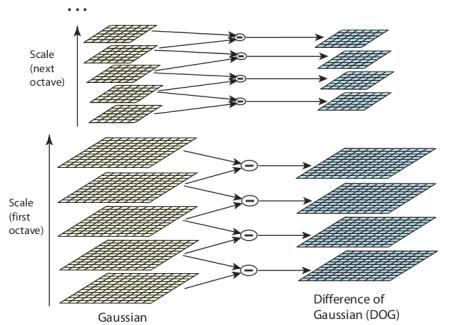
\includegraphics[width=.7\columnwidth]{sift.jpg}
   \caption{Difference of Gaussian}
   \label{fig:scale_gaussian} 
\end{figure}
Per ogni keypoint individuato è quindi definito un descrittore capace di descrivere i gradienti radiometrici nell’intorno del punto di interesse indipendentemente da rotazioni, variazioni di scala e cambiamenti di illuminazione. In base alla distanza euclidea fra questi vettori n-dimensionali è infine possibile individuare keypoints omologhi fra le immagini. Un esempio di punti di interesse estratti è mostrato in figura ~\ref{fig:keypoint}
\begin{figure}[H]
   \centering
   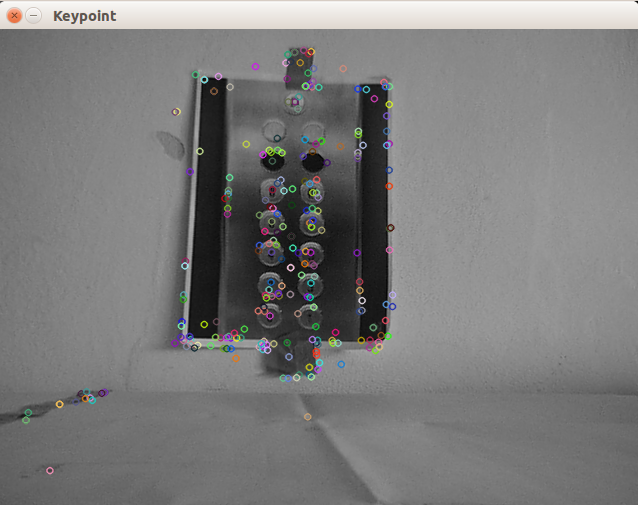
\includegraphics[width=1.\columnwidth]{keypoint.png}
   \caption{Keypoint}
   \label{fig:keypoint} 
\end{figure}
Il keypoint è quindi costituito dalle seguenti informazioni:
\begin{itemize}
\item posizione nel piano immagine
\item scala alla quale è stato rilevato il punto caratteristico
\item orientamento ossia la direzione principale del gradiente della regione nell'intorno del punto
\item descrittore che descrive in maniera univoca il punto caratteristico
\end{itemize}
Ad ogni frame vengono calcolati i keypoint e i relativi descrittori. Per ogni feature della prima immagine viene confrontato il suo descrittore con tutti i descrittori dei keypoint della seconda immagine. Il punto caratteristico con il descrittore che gli assomiglierà di più e che supera una soglia di somiglianza verrà definito come il punto corrispondente della prima immagine. In figura ~\ref{fig:matching} si può vedere un esempio di matching per il compito in esame.
\begin{figure}[H]
   \centering
   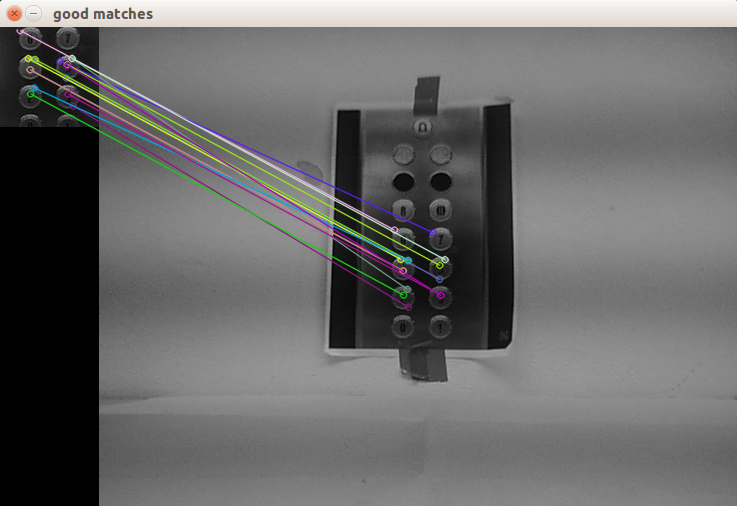
\includegraphics[width=1.\columnwidth]{match1.png}
   \caption{Match tra due frame consegutivi}
   \label{fig:matching} 
\end{figure} % Include the third content chapter
%!TEX root = pag0.tex
\chapter{Algoritmo}
\label{chapter4}

Lo scopo del progetto è di tracciare e stimare la posizione 3D del pulsante desiderato durante il moto del braccio utilizzando una camera monoculare. 
Come definito nel capitolo ~\ref{chapter1} la camera non fornisce informazioni sulla profondità. Per ottenere la posizione 3D date le informazioni 2D del pulsante si utilizza un algoritmo esterno detto PTAM. 
Per gestire i due algoritmi si utilizza il framework ROS atto a far comunicare più algoritmi contemporaneamente tramite l'invio di messaggi. 
In figura ~\ref{fig:struttura} si è schematizzata la struttura dell'algoritmo.
\begin{figure}[H]
   \centering
   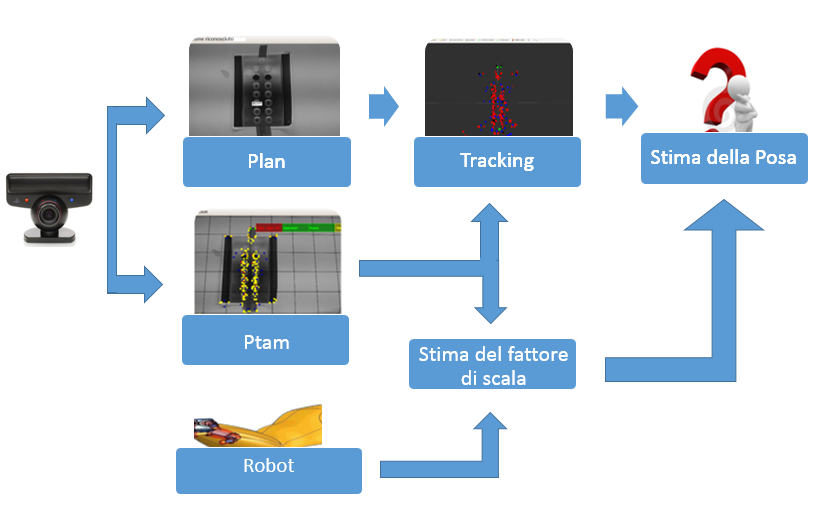
\includegraphics[width=0.9\columnwidth]{struttura.png} 
   \caption{Struttura dell'algoritmo sviluppato}
   \label{fig:struttura} 
\end{figure}
La prima parte è dedicata al riconoscimento delle forme geometriche nella scena e all'interazione con l'utente. La seconda parte è dedicata al tracking dell'oggetto desiderato nei successivi frame. L'ultima parte ricerca la posizione 3D del oggetto utilzzando sia le informazioni provenienti da PTAM, sia le informazioni sullo spostamento reale del robot. Nell'allegato ~\ref{Appendix} vengono mostrati le strutture degli algoritmi implementati.

\subsection{Fase di plan}
La telecamera invia lo streaming della scena al nodo Ros di PTAM e contemporaneamente invia un immagine statica, della stessa scena, al nodo da noi creato. Con questa immagine statica siamo in grado di riconoscere i contorni delle immagini tramite il filtro di Harris ~\cite{Harry}. Questo filtro è basato sull'approssimazione del auto-correlazione del gradiente in diverse direzioni. Per ogni contorno trovato si calcola i centri di massa e si verifica quale tra questi centri ha la minor distanza euclidea dal punto premuto dal utente. Dall'immagine si estrapola la zona dell'oggetto interessato e si calcolano le features e i relativi descrittori utilizzando il filtro Sift. Nella figura ~\ref{fig:fase_plan} si può vedere un esempio di questo algoritmo. 
\begin{figure*}
  \centering
   \subfigure[$Scena\_iniziale$]{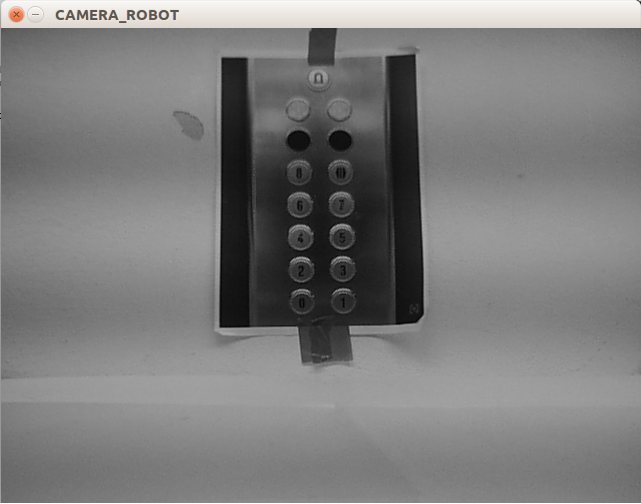
\includegraphics[width=.8\hsize]{fase1}\label{fig:scene}}
  \subfigure[$Bottone\_scelto$]{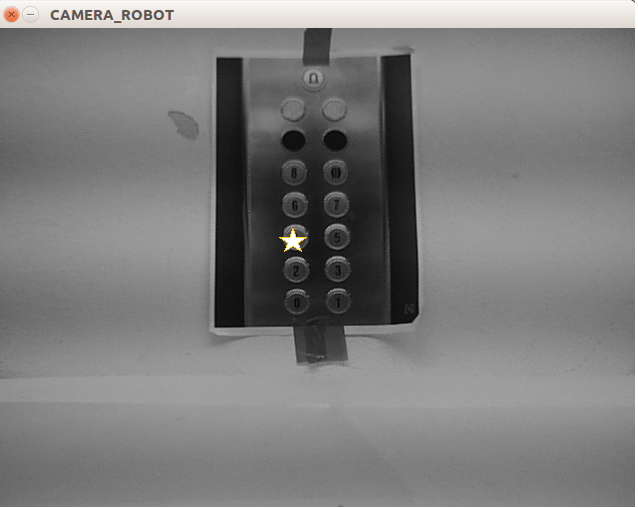
\includegraphics[width=.8\hsize]{bottonescelto}\label{fig:BottoneScelto}}
\end{figure*}
\begin{figure*}
  \centering  
  \subfigure[$Figure\_trovate$]{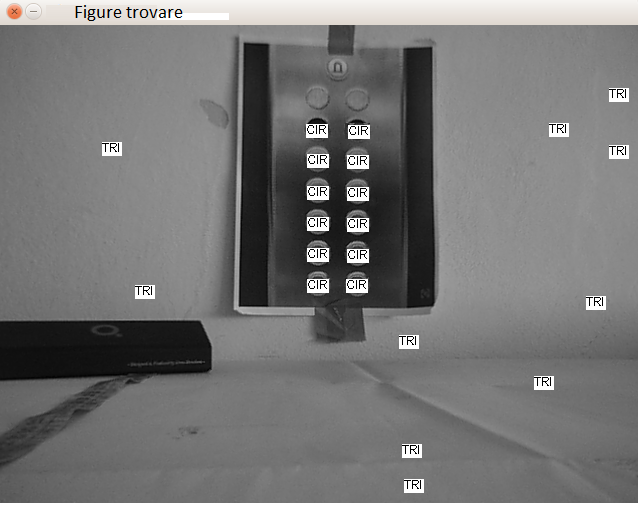
\includegraphics[width=.8\hsize]{figureTrovate}\label{fig:FigureTrovate}}
  \subfigure[$Bottone\_riconosciuto$]{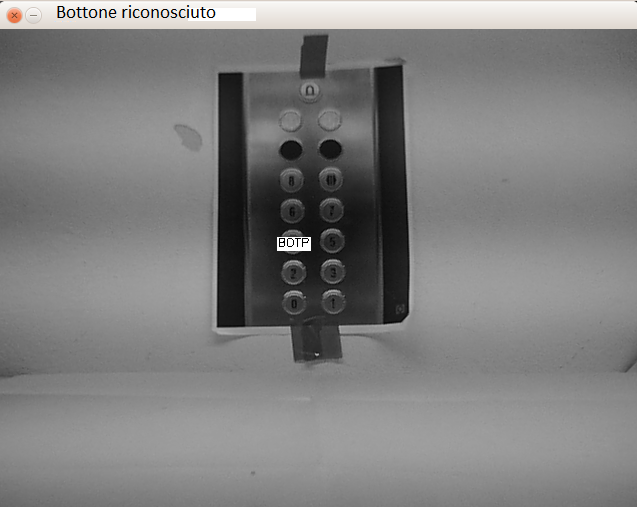
\includegraphics[width=0.8\hsize]{bottone_riconosciuto}\label{fig:bottonericonosciuto}}
  \caption{Esempio di ricerca del bottone selezionato}
  \label{fig:fase_plan}
\end{figure*}

\newpage
\subsection{Fase di tracking}
Quando il robot si muove invia un messaggio con la posa rispetto al frame precedente. In questo modo si tiene traccia dei reali spostamenti del robot. Nel nuovo frame si ricalcolano i descrittori dell'intera immagine e si calcola il match con le features del pulsante riconosciuto precedentemente. Il match è stato calcolato tramite il metodo FLANN acronimo di ~\emph{fast approximate nearest neighbor} ~\cite{FLANN}. Questo metodo consiste nel trovare i punti vicini tramite una ricerca randomica dell'albero creato. Utilizzando i migliori descrittori, che realizzano il matching, si calcola il centroide di questi punti. Questo nuovo punto rappresenta la posizione del pulsante nel nuovo frame. Ad ogni iterazione si esegue il matching con il pulsante trovato nella prima immagine.
In figura ~\ref{fig:fase_tracking} si può vedere un esempio del matching per il compito in esame. Come si può notare dalla figura ~\ref{fig:Matching} i descrittori trovati possono essere molti, anche distanti dalla zona di interesse. Per questa ragione si utilizza un controllo aggiuntivo basato sulle distanze per minimizzare questo numero. In figura ~\ref{fig:Good_matching} si mostrano i punti trovati utilizzando il controllo aggiuntivo. Questo controllo aggiuntivo fa in modo che la distanza euclidea dei punti del match non superi mai una soglia imposta. In questo modo riusciamo ad eliminare possibili outlier e a ridurre il campo di ricerca.     
\begin{figure*}
  \centering
  \subfigure[$Sift\_frame2$]{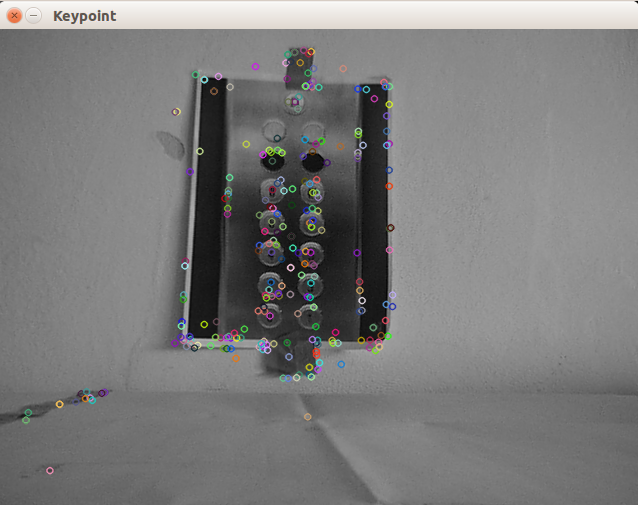
\includegraphics[width=.8\hsize]{keypoint}\label{fig:sift_scene2}}
  \subfigure[$Matching$]{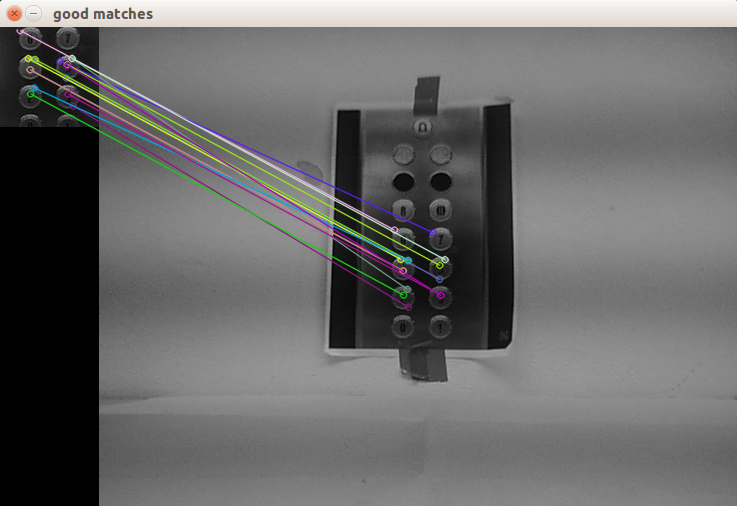
\includegraphics[width=.8\hsize]{match1}\label{fig:Matching}}
\end{figure*}
\begin{figure*}
  \centering  
  \subfigure[$Good\_matching$]{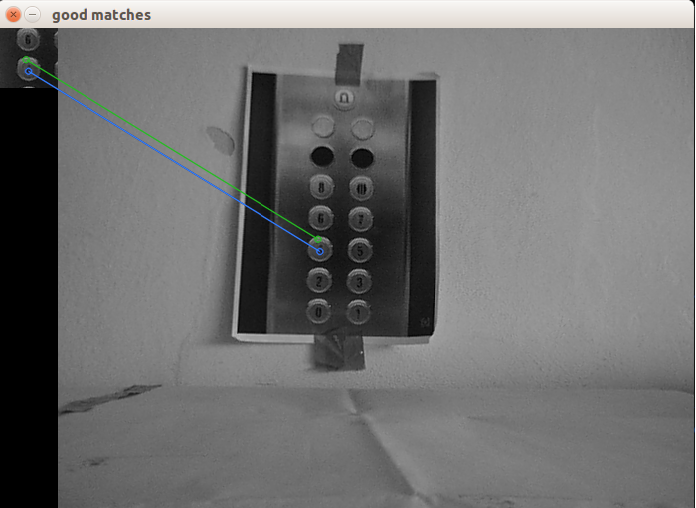
\includegraphics[width=.8\hsize]{goodmatch}\label{fig:Good_matching}}
  \subfigure[$Botton\_frame2$]{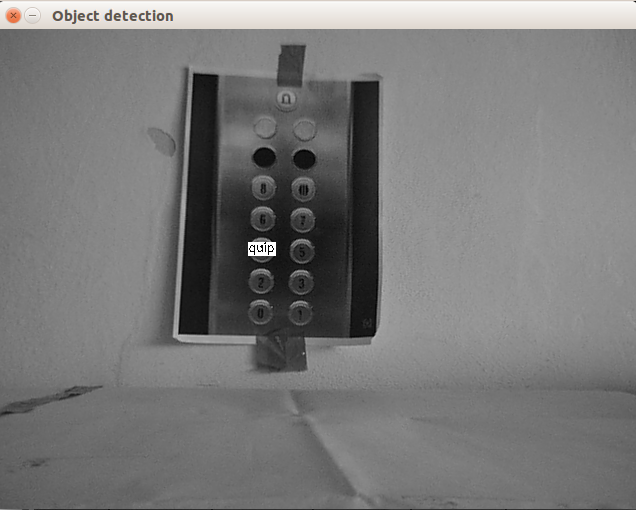
\includegraphics[width=.8\hsize]{bottone2frame}\label{fig:Botton_frame2}}
  \caption{Tracking del pulsante}
  \label{fig:fase_tracking}
\end{figure*}

\newpage
\subsection{Fase di interazione}
\subsubsection{Ptam}
Per spiegare come si è ottenuta la posa del pulsante rispetto alla telecamera, occorre spiegare come funziona l'algoritmo PTAM. Questo algoritmo è usato per la realtà aumentata e può essere riassunto da:
\begin{itemize}
\item Tracking delle features in ogni frame
\item Mapping delle features
\end{itemize}
Una mappa è un insieme di $M$ features rispetto al frame \lq \lq mondo\lq\lq $W$. Ogni features rappresenta un punto nel mondo 3D con coordinate $p_{jw} = (x_{jw} , y_{jw} , z_{jw}, 1)^t$ rispetto al frame W. La mappa è creata in fase di inizializzazione tramite la stereo visione. Come spiegato nel capitolo ~\ref{chapter2} la stereo visione è la stima della profondità tramite l'utilizzo di due immagini della stessa scena prese da angolazioni differenti. Durante la fase di inizializzazione la camera viene mossa sull'asse orizzontale, così facendo si tracciano le features durante lo spostamento e si stima la posizione 3D tramite algoritmi randomici. Un esempio di questa inizializzazione è mostrato in figura ~\ref{fig:fase_init}.
\begin{figure}[H]
   \centering
   \subfigure[$Fase\_init$]{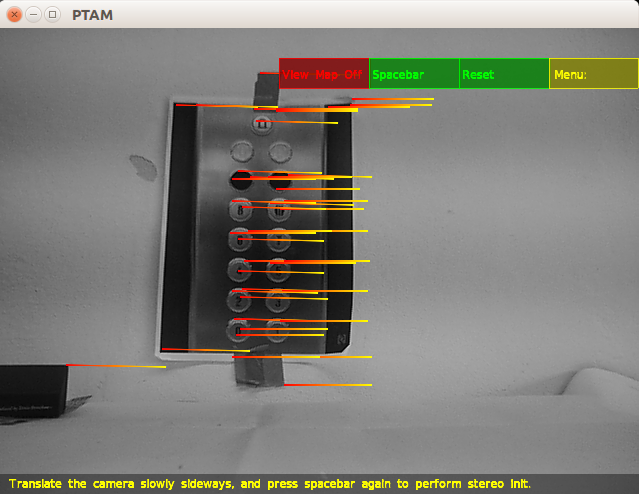
\includegraphics[width=.8\hsize]{ptaminit}\label{fig:fase_init}}
   \subfigure[$Ptam\_grid$]{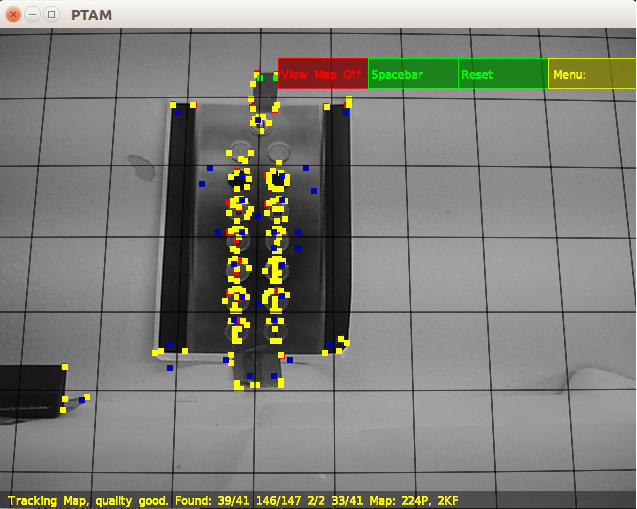
\includegraphics[width=.8\hsize]{ptamgrid}\label{fig:first_ptam_gird}}
   \caption{Fsse di inizializzazione di PTAM}
   \label{fig:fase_init} 
\end{figure}

Oltre alla posizione 3D delle features, figura ~\ref{fig:rviz_Fpoint}, rispetto al frame word questo algoritmo fornisce la posa della camera rispetto al frame W  ~\ref{fig:rviz_frame}. Questa posa è calcolata iterativamente minimizzando una funzione obbiettivo dato dall'errore di riproiezione nel piano immagine:
\begin{equation}
\mu = \argminB_\mu {\sum_{j \in S} Obj(\frac{|e_j|}{\sigma},\sigma_t)}
\label{eq:funzione obbiettivo}
\end{equation}
Dove $|e_t|$ è l'errore di riproiezione dato da:
\begin{equation}
e_t =  \left(\begin{array}{c} u_j \\ v_j \end{array} \right) - CamProj(exp(\mu)*E_{cw}*p_j)
\label{eq:errore di riproiezione}
\end{equation}
Il termine $CamProj($exp($\mu$)$ *E_{cw}*p_j)$ rappresenta il movimento della camera espresso come un vettore di $\mu$ usando una mappa esponenziale. 
\begin{figure*}
   \centering
    \subfigure[$Frame$]{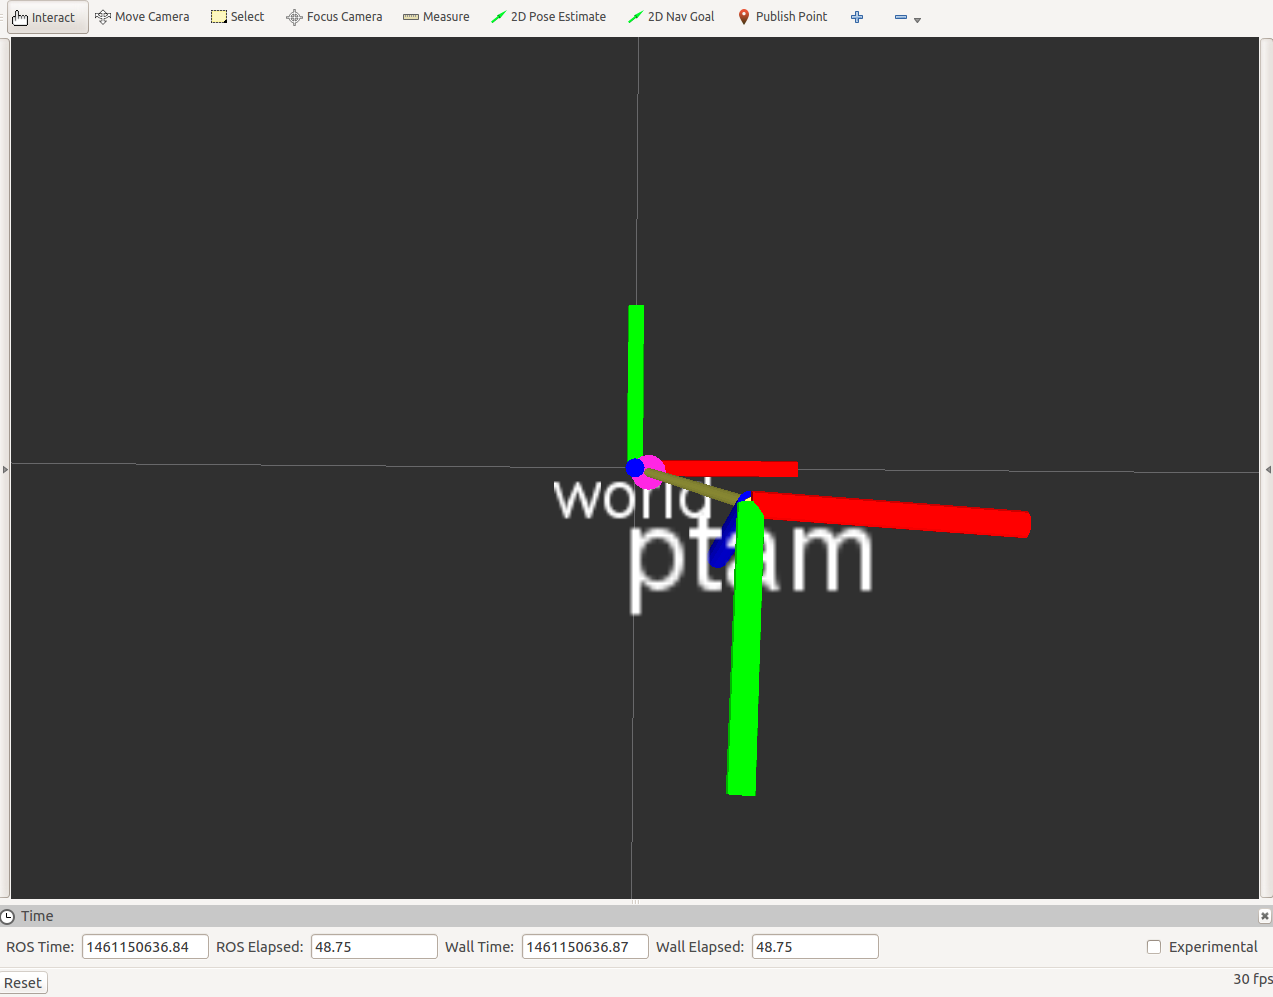
\includegraphics[width=.8\hsize]{rvizframe_}\label{fig:rviz_frame}}\\
   \subfigure[$Point\_W\_frame$]{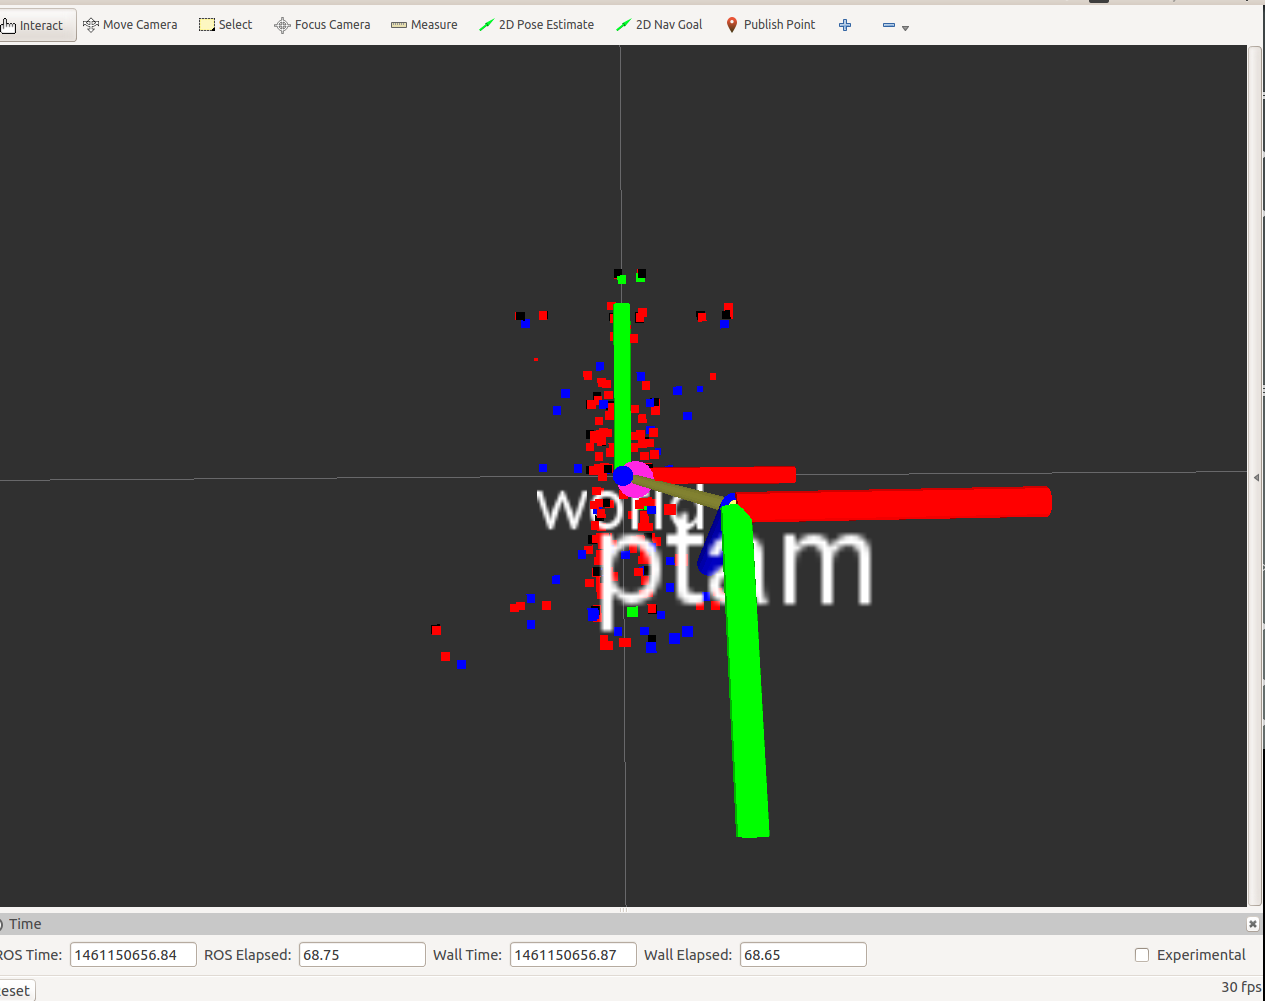
\includegraphics[width=.8\hsize]{rvizframepoint}\label{fig:rviz_Fpoint}}
\end{figure*}  
\begin{figure*}
 \centering
      \subfigure[$Point\_W\_frame$]{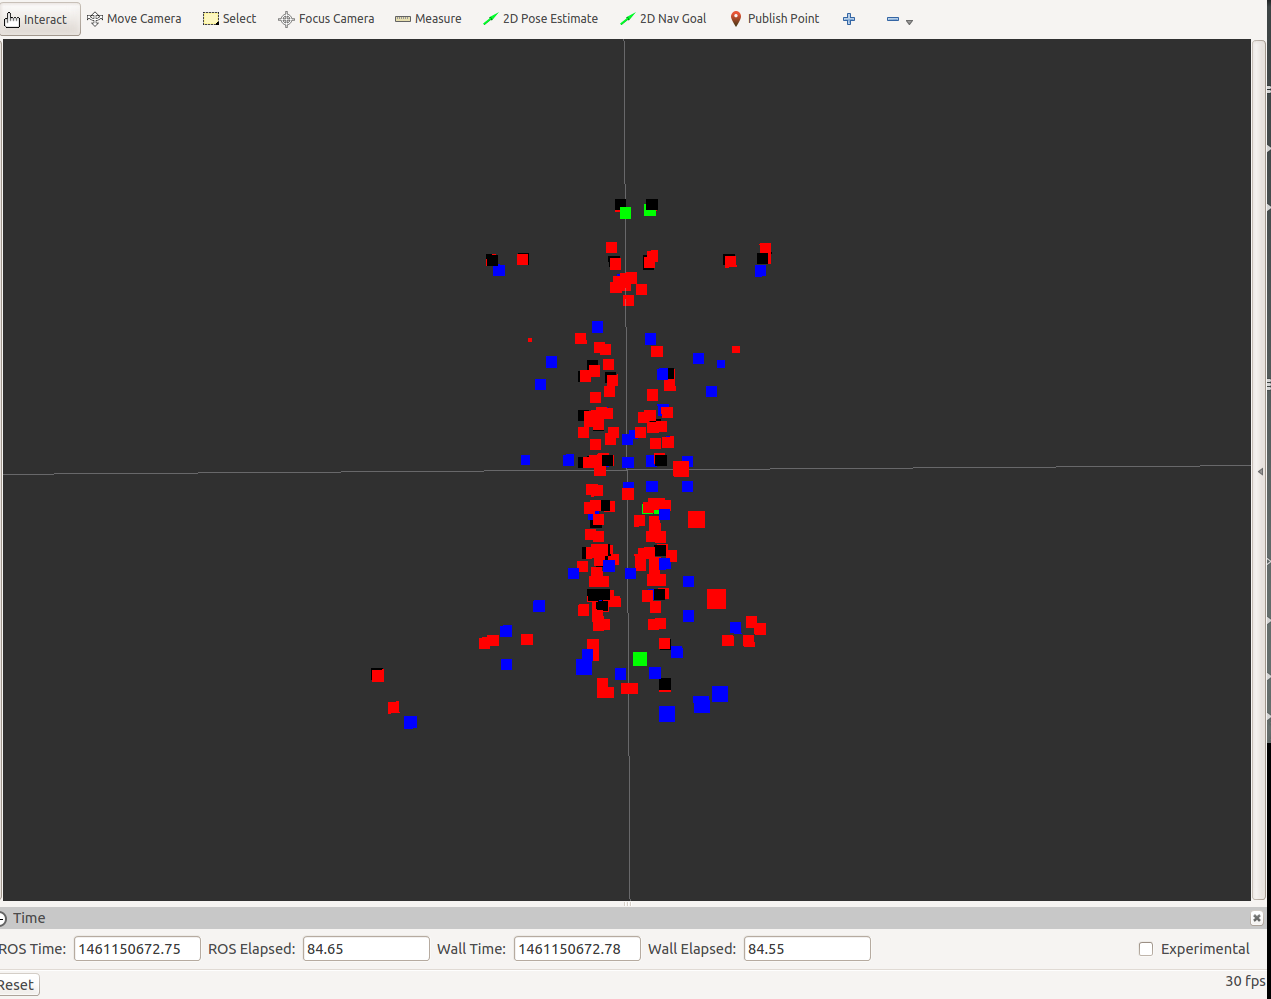
\includegraphics[width=.8\hsize]{rvizpoint}\label{fig:rviz_Fpoint}}
   \caption{Posizione delle features rispetto al word frame }
    \label{fig:rviz_point} 
\end{figure*}  
% \begin{figure}[H]
%    % \centering
%    \ContinuedFloat
%     \subfigure[$Point\_W\_frame$]{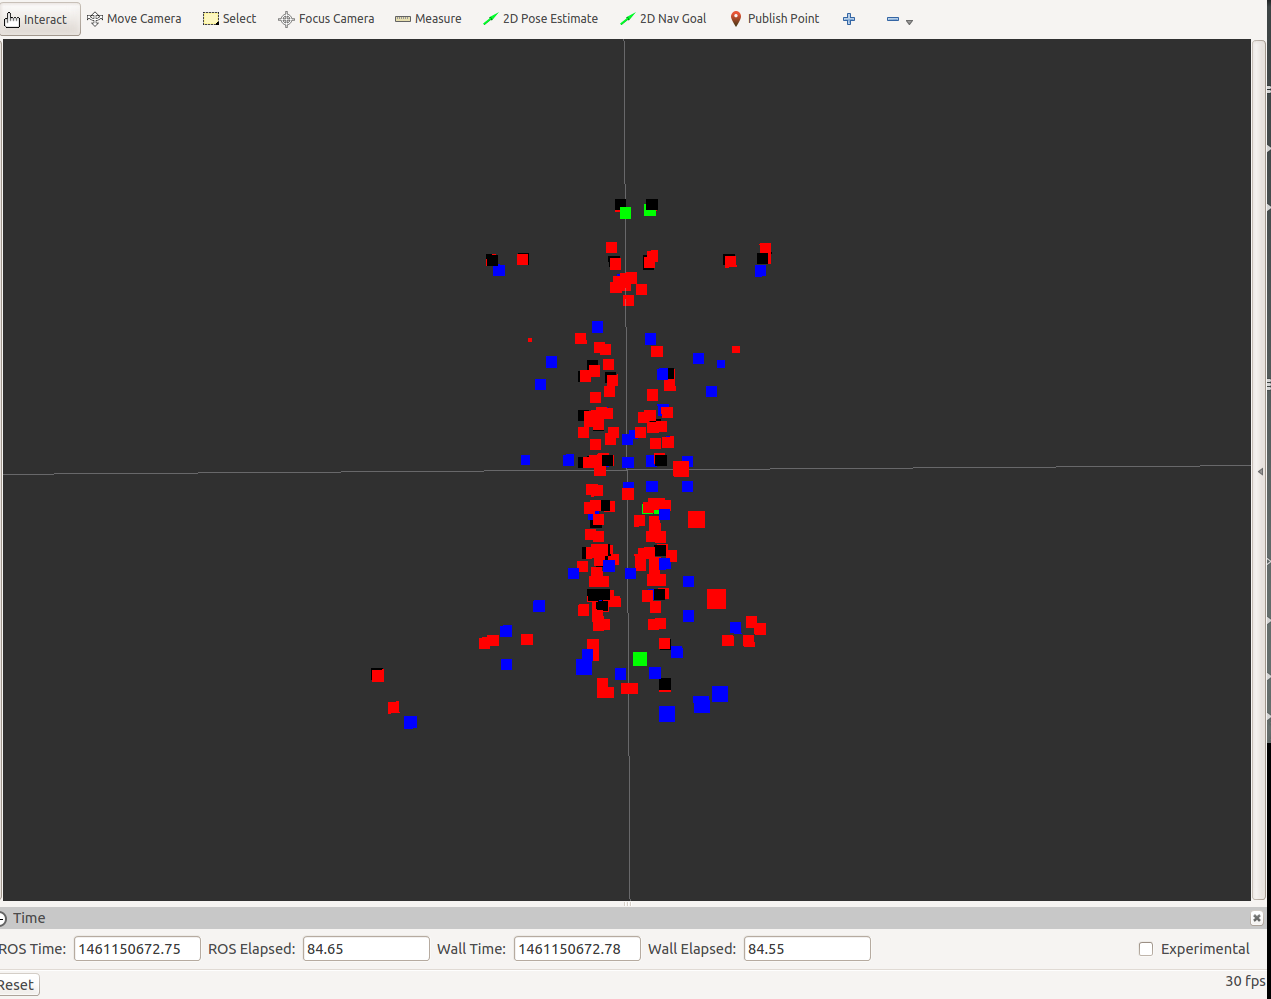
\includegraphics[width=.8\hsize]{rvizpoint}\label{fig:rviz_Fpoint}}
%    \caption{Posizione delle features rispetto al word frame }
%    \label{fig:rviz_point} 
% \end{figure}






\subsubsection{Stima del fattore di scala}
Come detto nel capitolo ~\ref{chapter1} questo algoritmo è soggetto ad un errore di scala. Se non correggessimo questo errore ci troveremmo in una posizione diversa rispetto alla posizione vera. Per questa ragione per correggere la scala si sono scritti due differenti metodi. 
Il primo metodo consente in un iterazione di stimare il valore della scala. Per questo metodo si utilizza il rapporto tra il reale spostamento del robot tra due sistemi di riferimento, e lo scostamento dato da Ptam.
\begin{equation}
s = \frac{Pr_{t-1} - Pr_{t}}{Pp_{t-1} - Pp_{t}}
\label{stima della scala primo metodo}
\end{equation}
Dove $Pr_{t-1} - Pr_{t}$ è lo spostamento reale del end-effector, mentre $Pp_{t-1} - Pp_{t}$ è lo spostamento secondo Ptam. Come vedremo nel capito ~\ref{chapter5} questo metodo è soggetto ad un errore di stima. Per ovviare a questo errore, si utilizzano dei metodi che permettono la convergenza della stima della scala al suo valore reale. Nel suo articolo Jacob Engel  ~\cite{scale} fornisce una stima dela fattore di scala utilizzando lo stimatore a massima verosimiglianza. Essenzialmente tale principio stabilisce di scegliere per un campione \underline{x} dato, quel valore di $\theta$ per cui massima era la probabilita' di estrarre proprio quel \underline{x}. Poiche' il logaritmo e' una funzione monotona, al posto del massimo di $L(\underline{x}, \theta)$ si preferisce cercare il massimo di $log L(\underline{x}, \theta)$. Dato una coppia di punti $(x_i, y_i)$, dove $x_i$ è la posizione affetta dal fattore di scala e $y_i$ è il valore reale, questi sono in relazione $x_i \approx \lambda y_i $. Se si ipotizza che il rumore di misura sia di tipo Gaussiano questi campioni possono essere scritti:
\begin{equation}
\begin{cases}
x_i \sim \Gamma(\lambda \mu_i, \sigma_x^2 I_{d*d})	\\
y_i \sim \Gamma(\mu_i, \sigma_y^2 I_{d*d})
\end{cases}
\label{rumore di misura}
\end{equation}
Dove $\mu_1 .... \mu_i$  $\epsilon$ $\Re^{d}$ rappresentano le vere ma ignote distanze, $\sigma_x^2$ e $\sigma_y^2$ rappresentano le varianze degli errori di misura.
Assumendo che le varianze siano note è possiile trovare una soluzione in forma chiusa dello stimatore minimizzando la funzione: 
\begin{equation}
L(\mu_1..\mu_n,\lambda)  \propto \frac{1}{2} \sum\limits_{i=1}^n (\frac{|| x_i - \lambda \mu_i ||^2}{\sigma_x^2}+ \frac{|| y_i - \mu_i|| ^2}{\sigma_y^2})
\label{funzione da minimizzare}
\end{equation}
Minimizzando per $\lambda$ è possibile trovare una soluzione unica
\begin{equation}
\lambda^* = \frac{s_{xx} - s_{yy} + sign(s_{xy}*\sqrt{(s_{xx} - s_{yy})^2 + 4*s_{xy}^2})}{2*\sigma_x^-1 * \sigma_y * s_{xy}}
\label{stima della scala per lo stimatore ML}
\end{equation}
Dove:
\begin{equation}
% \begin{cases}
s_{xx} = \sigma_y^2*\sum\limits_{i=1}^n x_i^t x_i	\qquad
s_{yy} = \sigma_x^2*\sum\limits_{i=1}^n y_i^t y_i	\qquad
s_{xy} = \sigma_y^2*\sigma_x^2 *\sum\limits_{i=1}^n x_i^t y_i^2
% \end{cases}
\label{}
\end{equation}
Questo metodo assicura la convergenza per un numero finito di passi. Nel capitolo ~\ref{chapter5} analizzeremo durante un esperimento i due metodi in esame.


\subsection{Posizione 3D del pulsante}
Per quanto detto finora PTAM tramite l'inizializzazione della mappa crea una collezione di punti 3D riferiti al frame mondo. La posizione delle features di interesse può essere acquisita da un utente esterno tramite la lettura del topic di riferimento. Questi punti sono inviati tramite un messaggio ROS in forma di point cloud\footnote{ Point cloud o nuvola di punti è un insieme di punti caratterizzati dalla loro posizione in un sistema di coordinate e da eventuali valori di intensità (colore, profondità, ecc.) ad essi associati. Esse servono solitamente come rappresentazione di strutture tridimensionali come oggetti o superfici } e, come si puo vedere da figura ~\ref{fig:point_cloud} rappresentano il 3D delle features trovate nella immagine.  
\begin{figure}[H]
   \centering
   \subfigure[$Features\_2d$]{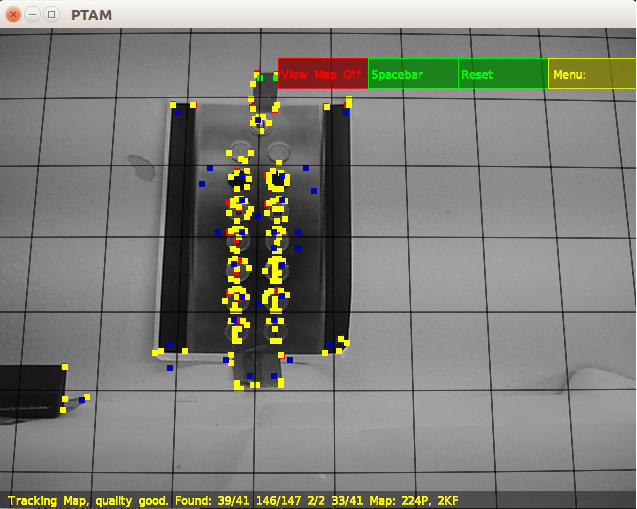
\includegraphics[width=.8\hsize]{ptamgrid}\label{fig:feature_2d}} 
   \subfigure[$Point\_cloud$]{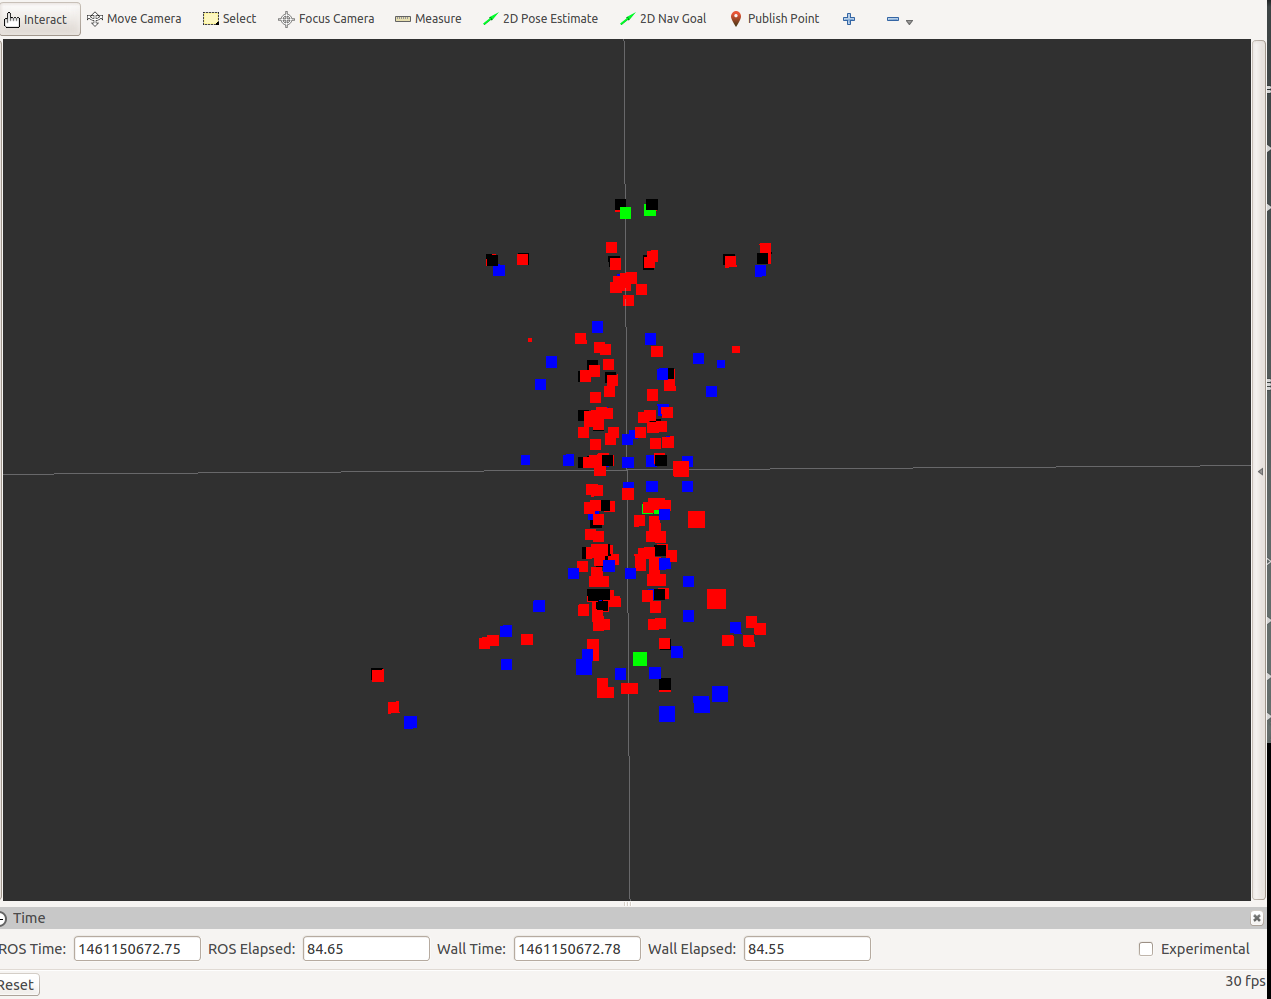
\includegraphics[width=.8\hsize]{rvizpoint}\label{fig:point_cloud}}
   \caption{Point cloud della mappa 3D}
   \label{fig:point_cloud} 
\end{figure}

Dalle informazioni della point cloud è possibile trovare le informazioni 2D riproiettando i punti nel piano immagine. Una volta che i punti vengono riproiettati si scelgono quelli più vicini al pulsante desiderato. Questa discriminazione viene fatta semplicemente calcolando tutte le distanze euclide dal pulsante. I punti scelti saranno quelli la cui distanza è minore di una soglia scelta, ci assicuriamo in questo modo di eliminare eventuali outlier presenti nel set di dati utilizzato. Grazie a questi punti è possibile trovare la posizione 3D del pulsante. Per ottenere questa infomazione si è deciso di fittare, tramite i minimi quadrati, un piano passante per questi punti. Utilizzando i parametri del piano assieme all'equazione ~\ref{eq:punto_immagine} è possibile trovare le coordinate 3D:
\begin{equation}
\begin{cases}
	a*X_c + b*Y_c + c*Z_c+ d = 0    \\
  	x_i = f_x * \frac{X_c}{Z_c}	+ c_x\\	
	y_i = f_y* \frac{Y_c}{Z_c} + c_y
 \end{cases}
 \label{sistema di equazione}
\end{equation}
Si hanno tre equazioni in tre incognite. 
\begin{equation}
\begin{cases}
	a*\frac{x_i - c_x}{f_x}*Z_c + b* \frac{y_i - c_y}{f_y}*Z_c + c*Z_c -d = 0   \\
  	X_c = \frac{x_i - c_x}{f_x} *Z_c\\	
	Y_c = \frac{y_i - c_y}{f_y} *Z_c
 \end{cases}
 \label{sistema di equazione}
\end{equation}
Da cui risolvendo per $Z_c$ si ottiene.
\begin{equation}
Z_c = \frac{d}{a*\frac{x_i - c_x}{f_x} + b* \frac{y_i - c_y}{f_y} +c }
\label{Profondita'}
\end{equation}
La posizione delle features che fornisce PTAM è rispetto al frame mondo, per i metodi implementati bisogna trasformarle nel sistema di riferimento camera tramite una trasformazione omogenea ~\ref{eq:wtocam}. Dove $T_c ^w$ rappresenta le cordinate del frame camera rispetto il frame mondo. 
\begin{equation}
P_c = T_c^w*P_w
\label{eq:wtocam}
\end{equation}
%!TEX root = pag0.tex
\chapter{Esperimenti}
\label{chapter5}
Nel capitolo ~\ref{chapter4} abbiamo parlato di due metodi per stimare il fattore di scala. Il primo è un metodo semplificato, dove la stima è fatta solo su di un campione e non c'è modo di verificare se questo valore è corretto. Se questa stima sbaglia, l'errore che genera viene portato avanti fino alla fine dell'esperimento. Come si vede in figura ~\ref{fig:1_metodo1} e ~\ref{fig:1_metodo2} la stima della scala con questo metodo, porti ad un errore massimo di stima della posizione di 1 cm per ogni spostamento effettuato.
\begin{figure}[H]
   \centering
   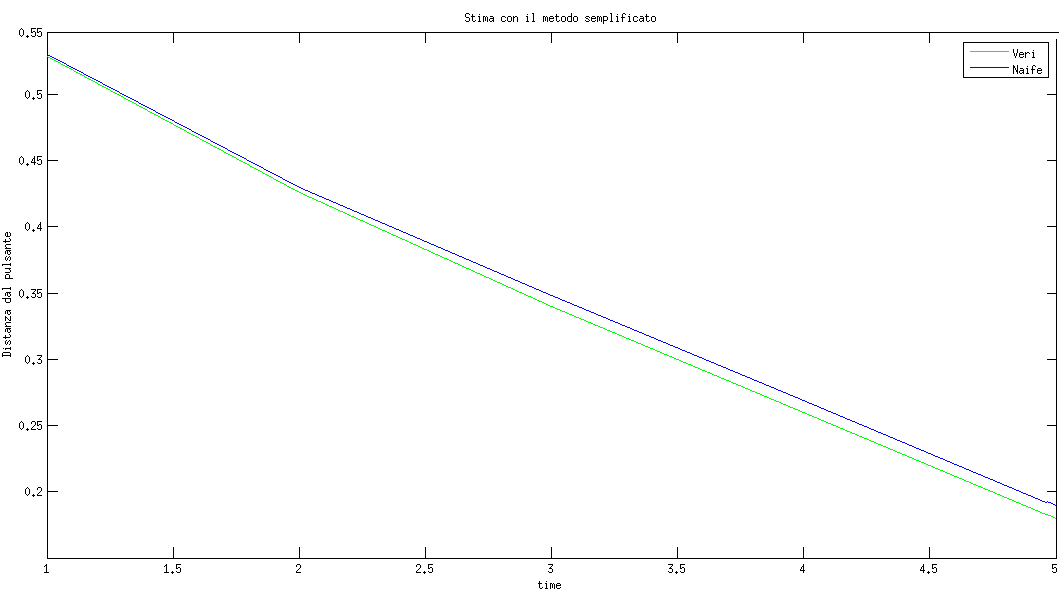
\includegraphics[width=1.\columnwidth]{naif25.png}
   \caption{Grafico dell'errore di stima della posa. In blu i dati stimati mentre in verde quelli reali}
   \label{fig:1_metodo1} 
\end{figure} 
\begin{figure}[H]
   \centering
   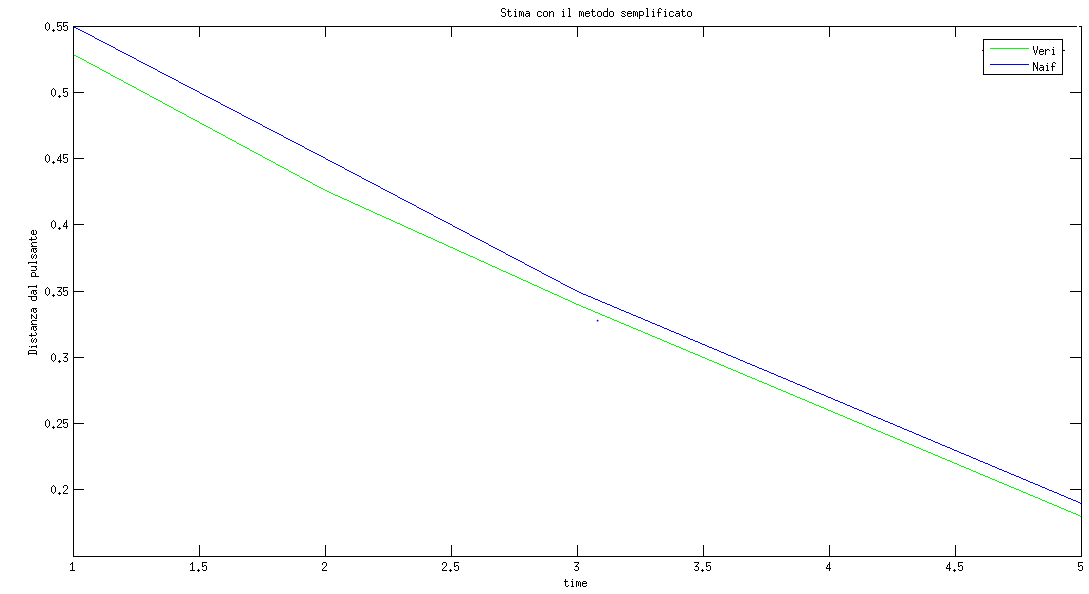
\includegraphics[width=1.\columnwidth]{naif28.png}
   \caption{Grafico dell'errore di stima della posa. In blu i dati stimati mentre in verde quelli reali}
   \label{fig:1_metodo2} 
\end{figure} 


Nel secondo metodo proposto invece, con l'utilizzo dello stimatore a massima verosomiglianza è possibile, utilizzando molti campioni, riuscire a far convergere l'errore di stima del fattore di scala al volore reale.
Per questo metodo occorro molti campioni. Per verificare la validità del metodo prendiamo un numero di campioni sufficientemente grande (maggiore di 500) di uno o più spostamenti. 
Per gli esperimenti si è scelto di utilizzare 1000 campioni di un unico spostamento, la convergenza è raggiunta se la differenza tra due campioni successivi è minore di 0.0001.
Nelle figure ~\ref{fig:mxli1} e ~\ref{fig:mxli2} possiamo vedere la convergenza della stima della scala per due esperimenti effettuati.
\begin{figure}[H]
   \centering
   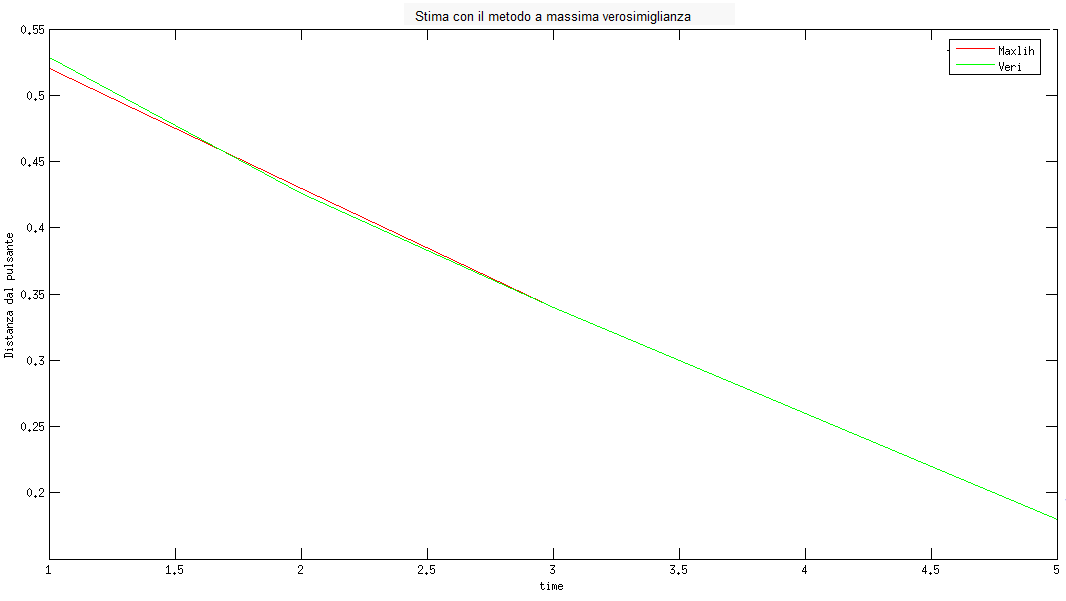
\includegraphics[width=1.\columnwidth]{maxlih24.png}
   \caption{Grafico dell'errore di stima della posa. In rosso i dati stimati mentre in verde quelli reali}
   \label{fig:mxli1} 
\end{figure} 
\begin{figure}[H]
   \centering
   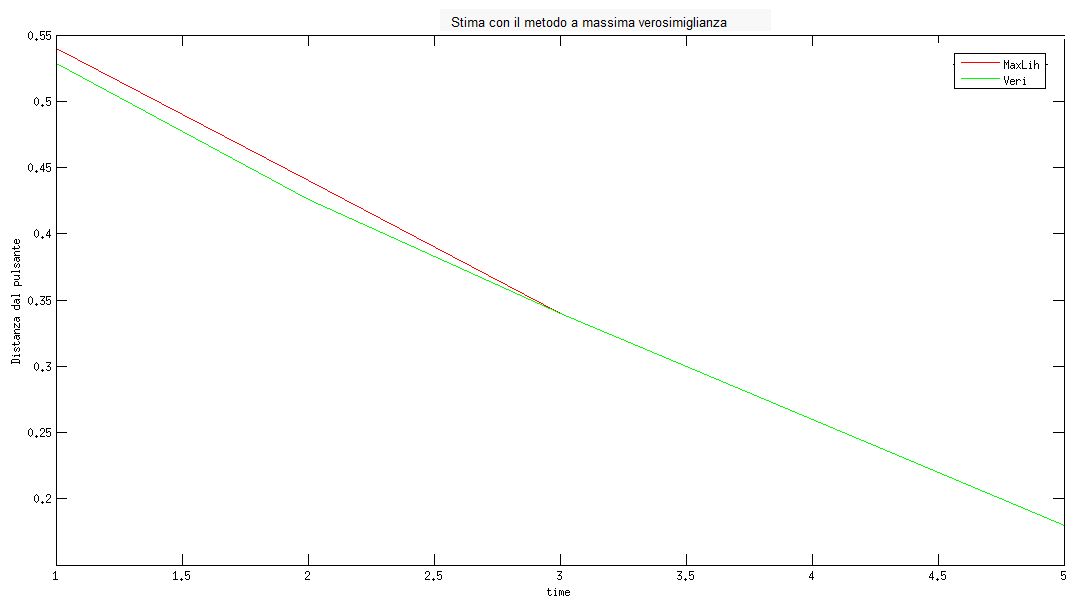
\includegraphics[width=1.\columnwidth]{maxlih28.png}
   \caption{Grafico della stima del valore di scala. In rosso i dati stimati mentre in verde quelli reali}
   \label{fig:mxli2} 
\end{figure} 
Nei due grafici sopra esposti si può vedere come la stima della scala con questo metodo, porti ad un errore massimo di qualche mm. 





\subsection{Confronto}
In figura  ~\ref{fig:confronto} mostriamo i confronti tra i due metodi per diversi set di dati.
\begin{figure*}
  \centering
  \subfigure[$confronto\_set1$]{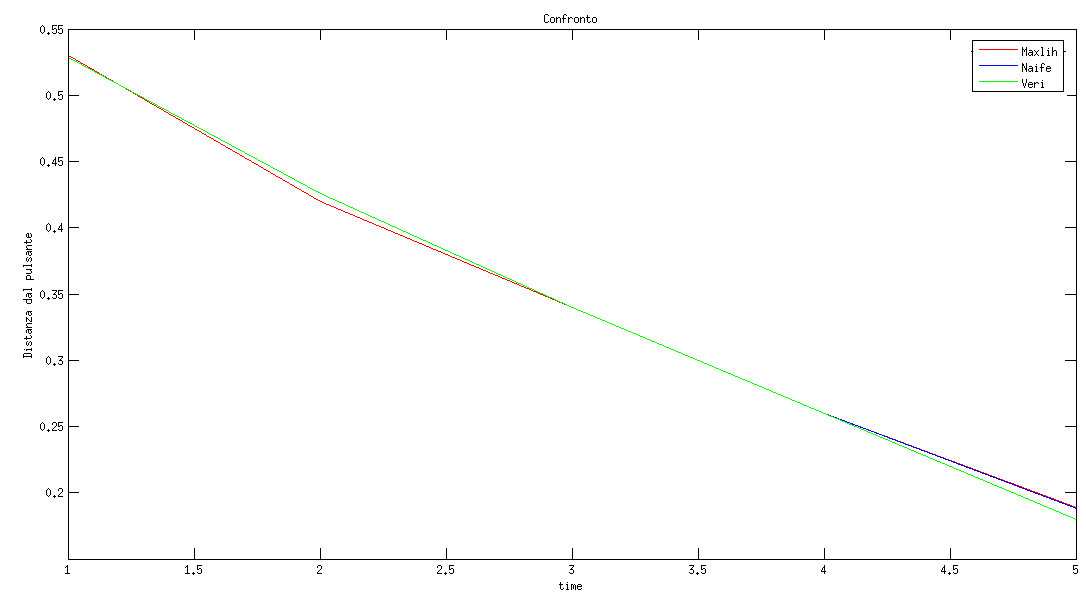
\includegraphics[width=1.\hsize]{Confrontoset24}\label{fig:confronto24}}
  \subfigure[$confronto\_set2$]{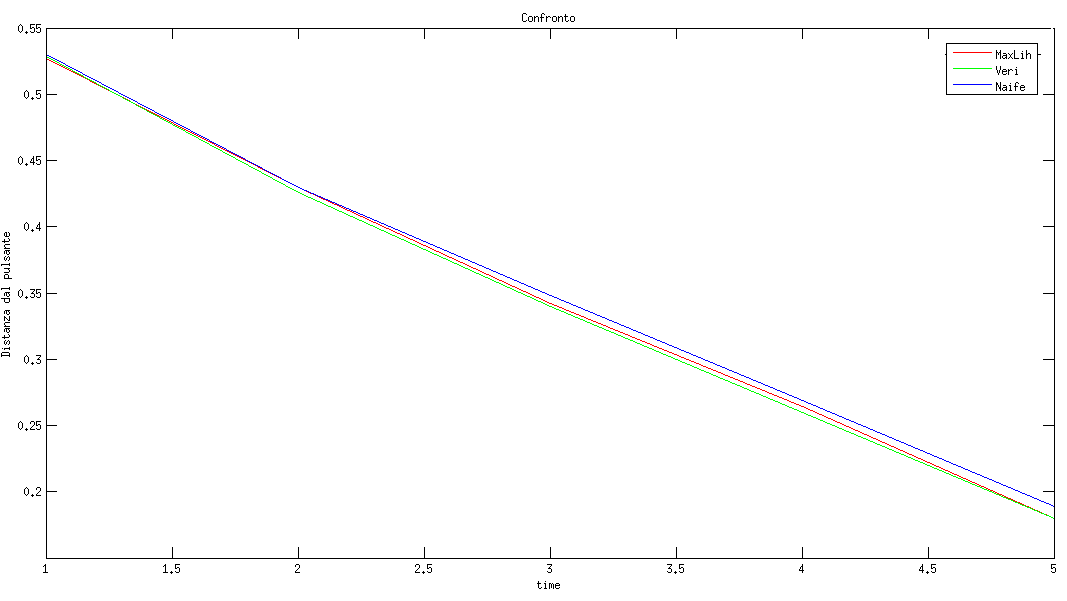
\includegraphics[width=1.\hsize]{Confrontoset25}\label{fig:confronto25}}
  % \subfigure[$confronto\_set3$]{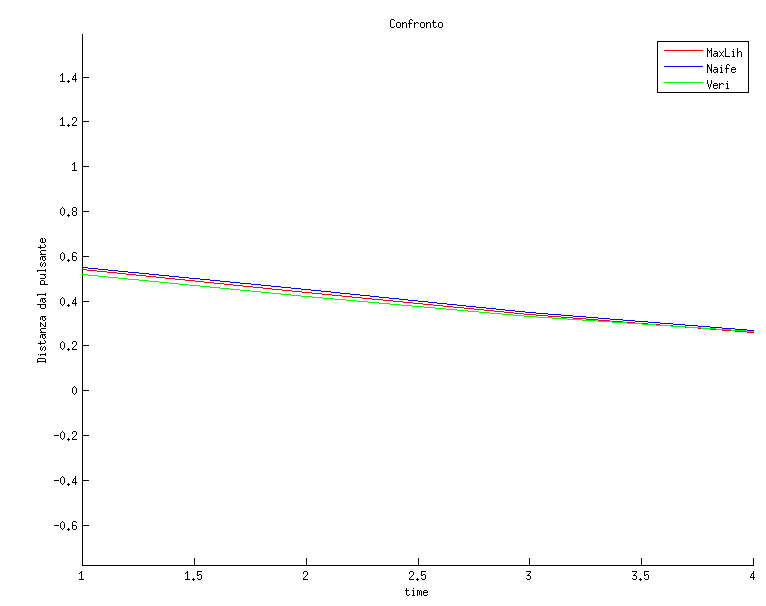
\includegraphics[width=1.\hsize]{Confronto28_1}\label{fig:confronto28}}
  \caption{Confronto tra i due metodi con la distanza effettiva}
  \label{fig:confronto}
\end{figure*}
Come possiamo vedere in figura ~\ref{fig:confronto} il metodo della massima verosimiglianza riesce a stimare meglio, nel lungo periodo, la posizione corretta della camera ottenendo un errore pari a 0.003 m. 

%!TEX root = pag0.tex
\chapter{Conclusioni}
\label{chapter6}
Come visto nel capitolo ~\ref{chapter5} entrambi i metodi comportano un minimo errore di stima della posizione. Questo errore di può essere causato da:
\begin{itemize}
\item nella fase di inizializzazione di Ptam. Non si raggiungono abbastanza features per creare una griglia stabile
\item nello spostamento per la stima della scala. Non si raggiungono o si superano i cm richiesti
\item nella fase di riproiezione dei punti.
\item ambiente circostante. 
\end{itemize}
Per rendere più stabile l'algoritmo si potrebbe utilizzare la dinamica del manipolare e un ulteriore controllo durante il percorso per correggere l'eventuale errore di posa.



% \backmatter

% \chapterstyle{default} % Reset the chapter style back to the default used for non-content chapters

\appendix
%!TEX root = pag0.tex

\chapter{Pseudo Codice}
\subsection{Fase di plan}

\begin{algorithm}
  \caption{Plan}\label{alg:Plan}
  \begin{algorithmic}[1]
    \State $Scena \gets TrovaContorni(p^{2D})$
    \State $PerogniContorno \gets CalcolaCentroDiMassa$
    % \State $vect_Objects \gets GetCluster(AllObjcets)$
      \If{$(PosizioneCentroDiMassa - Posizione Bottone Premuto < Soglia $} \Comment{Trovato pulsante desiderato}
      	\State $Scena \gets RitagliareImmagine(Posizione Bottone Premuto)$
            \State $ScenaTagliata \gets Sift$
      \Else 
      \Comment {Premere nuovamente il pulsante e far ripartire la procedura}
    \EndIf
    % \EndProcedure
  \end{algorithmic}
\end{algorithm}


\subsection{Fase di Tracking}

\begin{algorithm}
  \caption{Tracking}\label{alg:Tracking}
  \begin{algorithmic}[1]
    \State $Frame \gets Sift$
    \State $Match(FrameEBottonePremuto ) \gets Flann$
    \State $PerOgniKeypoint \gets CalcoloCentroide$
      \If{$(  PosizioneCentroide - Posizione Bottone Premuto  < Soglia $} \Comment{Feature valida}
      	\State $FeaturesValide \gets CalcoloCentroide $
      	\State $BottoneNellaSecondaImmagine  = Centroide $
      \Else 
      \Comment {Feature non valida}
    \EndIf
    % \EndProcedure
  \end{algorithmic}
\end{algorithm}


\subsection{Fase di Interazione}

\begin{algorithm}
  \caption{Interazione}\label{alg:Interazione}
  \begin{algorithmic}[1]
    \State $Punti3DFrameMondo \gets Ptam$
    \State $Punti3DFrameCamera \gets Trasformo(Punti3DFrameMondo)$
    \State $Scala \gets MessaggioDalNodoDiStima(Scala)$
     \State $Punti2D \gets Riproietto(Punti3D*Scala)$
     \If{$(  Posizione Punti2D - Posizione Bottone Premuto  < Soglia $} \Comment{Punti validi}
     \If{$(  PuntiValidi > 3 $} \Comment{Servono 3 punti per fittare il piano}
     \State $ParametriDelPiano \gets FitPiano(PuntiValidi)$
     \State $PosizioneBottone3D \gets ParametriDelPiano$
        \Else 
      \Comment {Impossibile trovare un piano}
      \EndIf
      % \If{$(  Posizione CalcoloCentroide - Posizione Bottone Premuto  < Soglia $} \Comment{Feature valida}
      	% \State $FeaturesValide \gets CalcoloCentroide $
      \Else 
      \Comment {Punti non validi}
    \EndIf
    % \EndProcedure
  \end{algorithmic}
\end{algorithm}


\subsection{Stima del fattore di scala}

\begin{algorithm}
  \caption{Scala}\label{alg:scala}
  \begin{algorithmic}[1]
    \State $PosizioneRobotPtamAttuale \gets Ptam$
    \State $MovimentoRobotReale \gets Robot$
    \State $PosizioneRobotPtamPrecedente $\Comment{Salvata ad ogni spostamento}
    \State $MovimentoRobotPtam \gets PosizioneRobotPtamPrecedente*PosizioneRobotPtamAttuale$
     \If{$Vect(MovimentoRobotPtam).size() > 1000 $} \Comment{Se si è preso abbastanza campioni}
     % \If{$(  Punti validi > 3 $} \Comment{Servono 3 punti per fittare il piano}
    \State $Scala \gets MassimaVerossimiglianza(MovimentoRobotPtam, MovimentoRobotReale)$
        \State $InvioMessaggio \gets scala$
     \Else 
      \Comment {wait}

    % 
    \EndIf
    % \EndProcedure
  \end{algorithmic}
\end{algorithm}

% \chapter{Pseudo Codice}
\label{Appendix}
% %!TEX root = pag0.tex

\chapter{Pseudo Codice}
\subsection{Fase di plan}

\begin{algorithm}
  \caption{Plan}\label{alg:Plan}
  \begin{algorithmic}[1]
    \State $Scena \gets TrovaContorni(p^{2D})$
    \State $PerogniContorno \gets CalcolaCentroDiMassa$
    % \State $vect_Objects \gets GetCluster(AllObjcets)$
      \If{$(PosizioneCentroDiMassa - Posizione Bottone Premuto < Soglia $} \Comment{Trovato pulsante desiderato}
      	\State $Scena \gets RitagliareImmagine(Posizione Bottone Premuto)$
            \State $ScenaTagliata \gets Sift$
      \Else 
      \Comment {Premere nuovamente il pulsante e far ripartire la procedura}
    \EndIf
    % \EndProcedure
  \end{algorithmic}
\end{algorithm}


\subsection{Fase di Tracking}

\begin{algorithm}
  \caption{Tracking}\label{alg:Tracking}
  \begin{algorithmic}[1]
    \State $Frame \gets Sift$
    \State $Match(FrameEBottonePremuto ) \gets Flann$
    \State $PerOgniKeypoint \gets CalcoloCentroide$
      \If{$(  PosizioneCentroide - Posizione Bottone Premuto  < Soglia $} \Comment{Feature valida}
      	\State $FeaturesValide \gets CalcoloCentroide $
      	\State $BottoneNellaSecondaImmagine  = Centroide $
      \Else 
      \Comment {Feature non valida}
    \EndIf
    % \EndProcedure
  \end{algorithmic}
\end{algorithm}


\subsection{Fase di Interazione}

\begin{algorithm}
  \caption{Interazione}\label{alg:Interazione}
  \begin{algorithmic}[1]
    \State $Punti3DFrameMondo \gets Ptam$
    \State $Punti3DFrameCamera \gets Trasformo(Punti3DFrameMondo)$
    \State $Scala \gets MessaggioDalNodoDiStima(Scala)$
     \State $Punti2D \gets Riproietto(Punti3D*Scala)$
     \If{$(  Posizione Punti2D - Posizione Bottone Premuto  < Soglia $} \Comment{Punti validi}
     \If{$(  PuntiValidi > 3 $} \Comment{Servono 3 punti per fittare il piano}
     \State $ParametriDelPiano \gets FitPiano(PuntiValidi)$
     \State $PosizioneBottone3D \gets ParametriDelPiano$
        \Else 
      \Comment {Impossibile trovare un piano}
      \EndIf
      % \If{$(  Posizione CalcoloCentroide - Posizione Bottone Premuto  < Soglia $} \Comment{Feature valida}
      	% \State $FeaturesValide \gets CalcoloCentroide $
      \Else 
      \Comment {Punti non validi}
    \EndIf
    % \EndProcedure
  \end{algorithmic}
\end{algorithm}


\subsection{Stima del fattore di scala}

\begin{algorithm}
  \caption{Scala}\label{alg:scala}
  \begin{algorithmic}[1]
    \State $PosizioneRobotPtamAttuale \gets Ptam$
    \State $MovimentoRobotReale \gets Robot$
    \State $PosizioneRobotPtamPrecedente $\Comment{Salvata ad ogni spostamento}
    \State $MovimentoRobotPtam \gets PosizioneRobotPtamPrecedente*PosizioneRobotPtamAttuale$
     \If{$Vect(MovimentoRobotPtam).size() > 1000 $} \Comment{Se si è preso abbastanza campioni}
     % \If{$(  Punti validi > 3 $} \Comment{Servono 3 punti per fittare il piano}
    \State $Scala \gets MassimaVerossimiglianza(MovimentoRobotPtam, MovimentoRobotReale)$
        \State $InvioMessaggio \gets scala$
     \Else 
      \Comment {wait}

    % 
    \EndIf
    % \EndProcedure
  \end{algorithmic}
\end{algorithm}




% \backmatter
% \addlibresource{bibliography}
\bibliographystyle{IEEEtran}
\bibliography{bibliography}
% \begin{thebibliography}{}
% \bibliography{biblio}
% \bibliographystyle{unsrt}
% \bibliography{bibliography}
% \end{thebibliography}

% \end{flushleft}

\end{document}

